\section{设计验证}
\begin{center}
    (该章满分20分)
\end{center}

\subsection{仿真验证}

选取2.3节中的任意两条机器指令,给出机器码格式,建立testbench文件,进行波形仿真。给出测试结果(波形图需要截屏)。

这里所给出的Processor已经被修改过了,主要是为了可以直观的看到执行机器码之后对寄存器的修改。

\begin{minted}{gas}
30f20a00000000000000 |   irmovq $10,%rdx
30f00300000000000000 |   irmovq  $3,%rax
6020                 |   addq %rdx,%rax
\end{minted}

\begin{minted}{verilog}
module testbench( );
    parameter RUN_MODE = 2'h0;
    parameter RESET_MODE = 2'h1;
    parameter DOWNLOAD_MODE = 2'h2;
    parameter UPLOAD_MODE = 2'h3;
    
    reg clock = 0;
    reg [2:0] mode = RESET_MODE;
    reg [63:0]uaddr = 0;
    reg [63:0]idata = 1;
    wire [63:0]rax;
    wire [63:0]rdx;
    
    always begin
        clock = 1;
        # 5;
        clock = 0;
        # 5;
    end
    
    //30f20a00000000000000 |   irmovq $10,%rdx
    //30f00300000000000000 |   irmovq  $3,%rax
    //6020                 |   addq %rdx,%rax
    
    initial begin
    #20 mode <= DOWNLOAD_MODE;
    uaddr <= 0;
    idata <= 64'h00000000000af230;
    #20;
    uaddr <= 8;
    idata <= 64'h00000003f0300000;
    #20;
    uaddr <= 16;
    idata <= 64'h000206000000000;
    #20;
    uaddr <= 24;
    idata <= 64'h0000000000000000;
    #20 mode <= RESET_MODE;
    #20 mode <= RUN_MODE;
    end
    
    Processor p(mode,uaddr,idata,rax,rdx,clock);

endmodule
\end{minted}

\begin{figure}
    \centering
    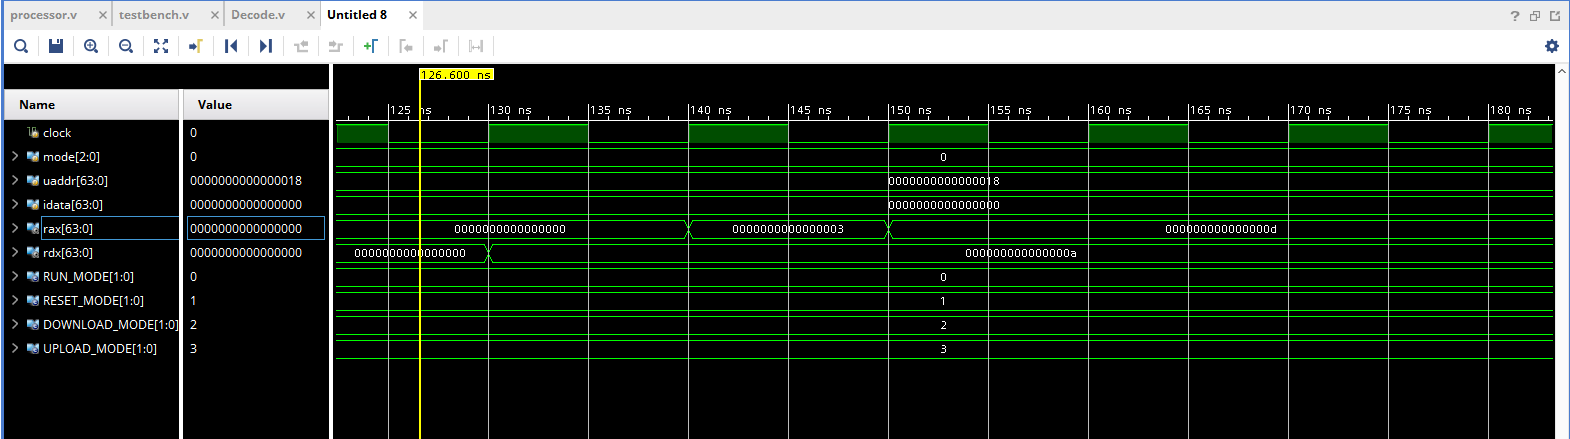
\includegraphics[width=0.7\linewidth]{figures/Sim}
    \caption{仿真波形}
    \label{fig:sim}
\end{figure}


\subsection{综合(synthesis)验证}
\begin{center}
    (选做,加分项,最多加分值为作业项总成绩的5分,作业项分值加满为止)
\end{center}

以2.3节中的程序为例,写出对应机器码格式,在某FPGA实验台上验证。

\section{总结}
\subsection{请总结本次实验的收获}
\begin{enumerate}
    \item 重新复习了vivado和verilog相关知识
    \item 对CPU顺序处理器的内部结构和运转过程有了更加深入的了解
    \item 在对SEQ不断修改调整的过程中加深了对CPU功能及与内存关系的理解
\end{enumerate}

\subsection{请给出对本次实验内容的建议}
希望可以第一时间给出参考资料。